\documentclass[11pt,a4paper]{article}
\pdfminorversion=7
\pdfsuppresswarningpagegroup=1
\usepackage[utf8]{inputenc}
\usepackage[T1]{fontenc}
\usepackage{lmodern}
\usepackage[margin=24mm]{geometry}
\usepackage{graphicx}
\usepackage{amsmath}
\usepackage[hidelinks]{hyperref}
\graphicspath{{figures/}}
\setlength{\parindent}{0pt}
\setlength{\parskip}{0.52em}
\setlength{\emergencystretch}{3em}
\newcommand{\dIF}{\ensuremath{\Delta\mathrm{IF}}}
\title{\textbf{Additional file 1: supplementary figures}\\\large A systematic framework for detecting transient developmental transcript-usage patterns identifies an E15.5-centred midbrain candidate landscape}
\author{Robin Gounder and Russell Hamilton}
\date{}

\begin{document}
\maketitle

\section*{Supplementary figures}
\setcounter{figure}{0}
\renewcommand{\thefigure}{S\arabic{figure}}
\renewcommand{\theHfigure}{S\arabic{figure}}

\begin{figure}[htbp]
\centering
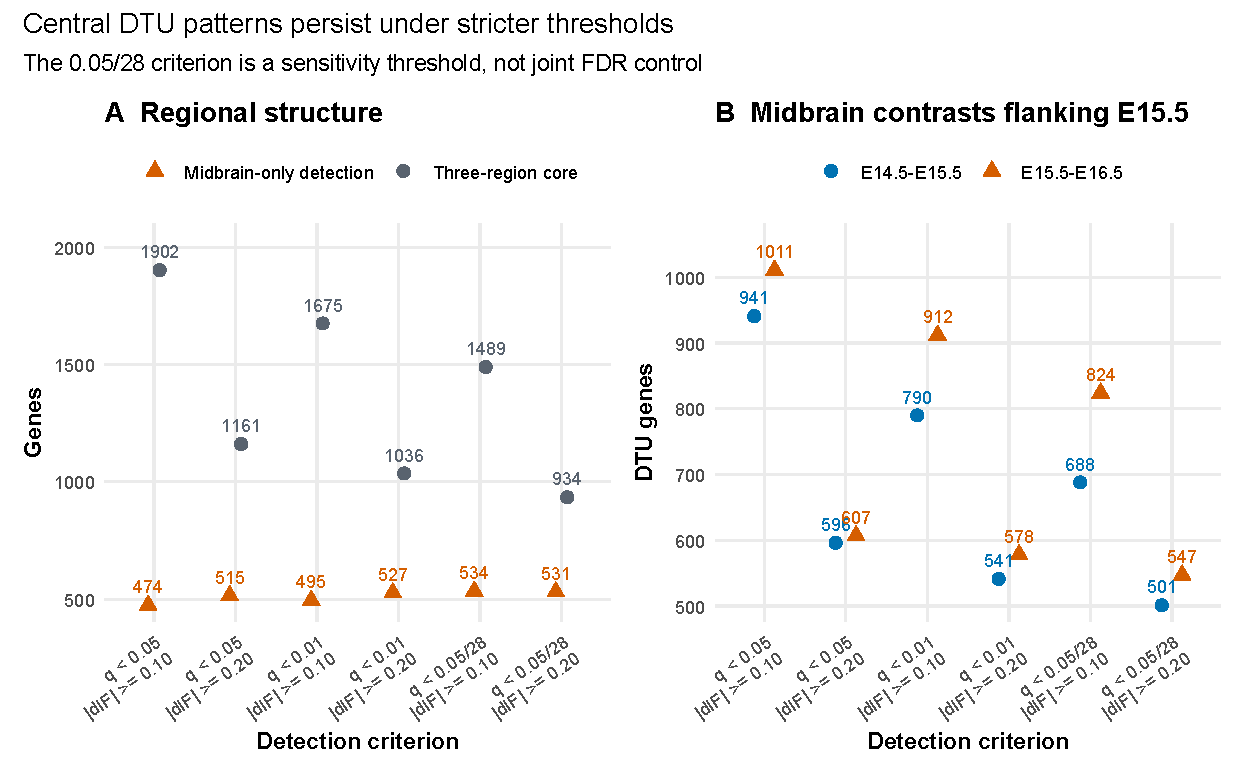
\includegraphics[width=\textwidth]{figureS2_repaired_thresholds.pdf}
\caption{\textbf{Threshold sensitivity of the regional DTU landscape.} Each point is a unique-gene count under the q-value and absolute change in relative transcript fraction ($|\dIF|$) criterion printed on the x-axis; numbers above points give the exact counts. (A) Circles denote genes detected in forebrain, hindbrain and midbrain, and triangles genes detected only in midbrain, after taking the union across all 28 within-region temporal contrasts. (B) Circles and triangles denote genes detected in the E14.5--E15.5 and E15.5--E16.5 midbrain contrasts, respectively. The $0.05/28$ q-value cutoff is a conservative one-at-a-time sensitivity threshold and does not constitute joint FDR control across contrasts.}
\label{fig:thresholds}
\end{figure}

\begin{figure}[htbp]
\centering
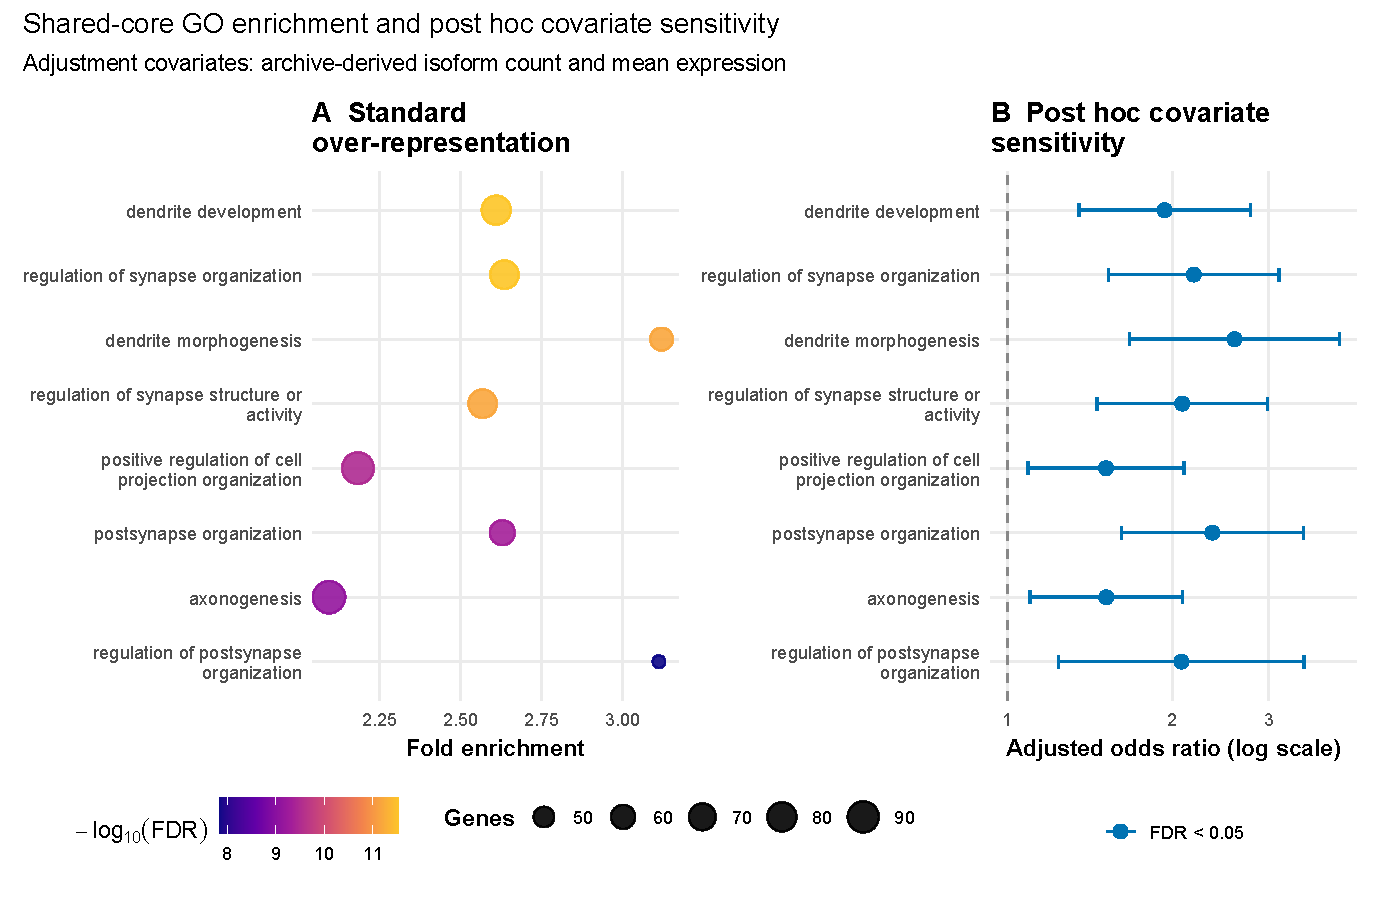
\includegraphics[width=\textwidth]{figureS4_repaired_go_enrichment.pdf}
\caption{\textbf{Shared-core Gene Ontology enrichment and covariate sensitivity.} The analysed set is the 1,902-gene three-region DTU core and the background is the 18,346-gene expressed universe. (A) The eight leading Biological Process terms from the clusterProfiler over-representation analysis. The x-axis is fold enrichment, point size is the number of shared-core genes annotated to the term and colour is $-\log_{10}$ of the Benjamini--Hochberg-adjusted enrichment $P$-value. (B) Post hoc logistic-regression estimates for the same eight terms after adjustment for $\log(1+\text{detectable isoform count})$ and $\log(1+\text{mean expression})$. Points are adjusted odds ratios, horizontal lines are 95\% confidence intervals, the dashed line marks an odds ratio of 1 and blue denotes q-value $<0.05$ after Benjamini--Hochberg adjustment across the eight models.}
\label{fig:go}
\end{figure}

\begin{figure}[htbp]
\centering
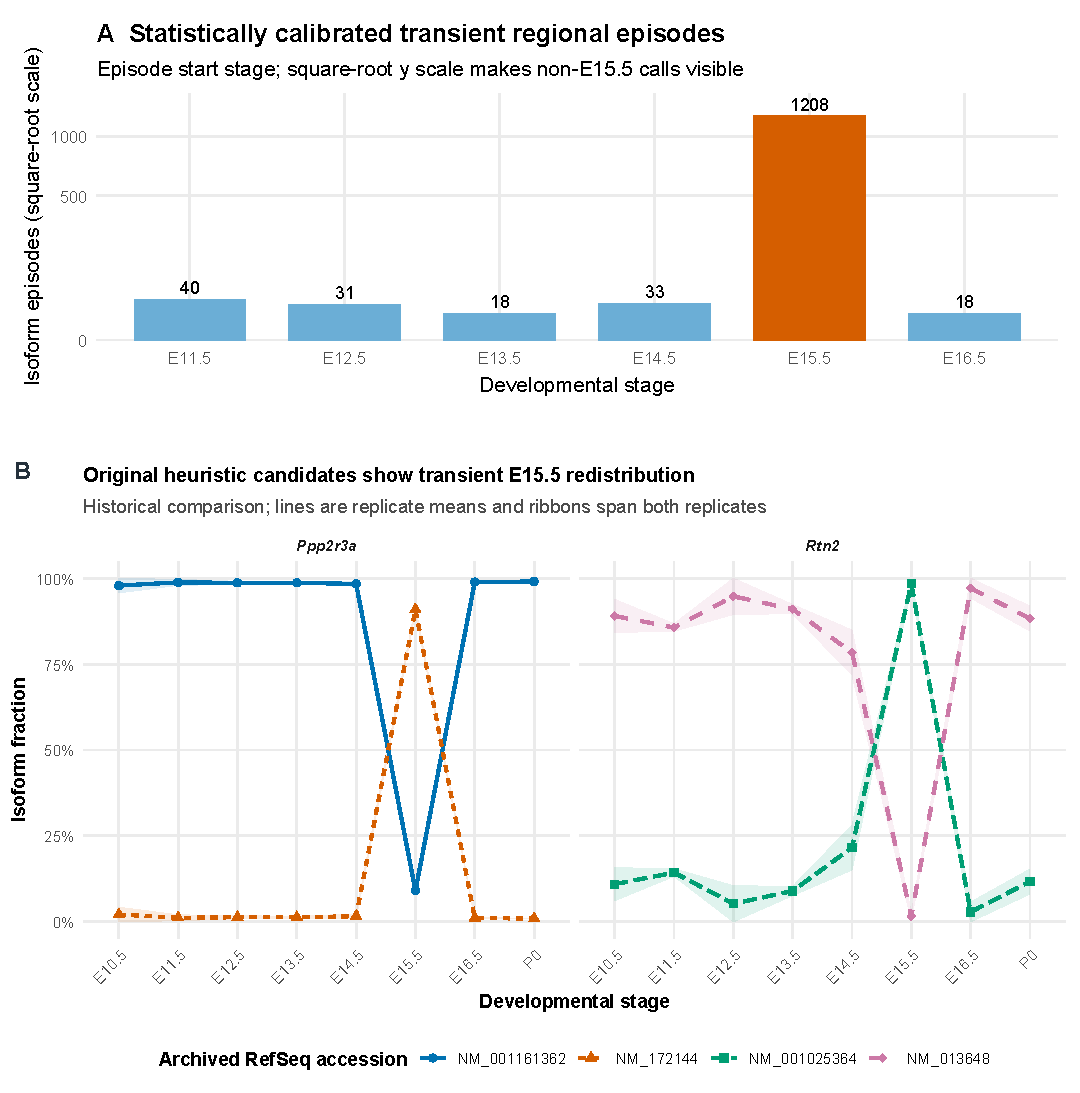
\includegraphics[width=\textwidth]{figure03_repaired_transient_episodes.pdf}
\caption{\textbf{Systematic episodes and original delayed-response examples.} The upper panel gives the number of replicate-consistent diverge--reconverge episodes beginning at each embryonic stage; bar labels are raw counts and the y-axis uses a square-root scale so that non-E15.5 calls remain visible. The middle block shows stage-mean transcript fractions for the six programmatically highest-ranked systematic reciprocal pairs: solid lines are midbrain, dashed lines the forebrain/hindbrain mean, and orange/blue denote the transcript higher/lower in midbrain at E15.5. The higher/lower accessions are \textit{Ntrk2} NM\_008745/NM\_001025074, \textit{Scg3} NM\_009130/NM\_001164790, \textit{Tecr} NM\_134118/NM\_027179, \textit{Armc8} NM\_028768/NM\_001166138, \textit{Bin1} NM\_001083334/NM\_009668 and \textit{Gpm6a} NM\_001253754/NM\_153581. The lower block shows the original heuristic candidates \textit{Ppp2r3a} (NM\_001161362 and NM\_172144) and \textit{Rtn2} (NM\_001025364 and NM\_013648); lines are replicate means and ribbons span the two replicate values. All trajectories cover E10.5--P0 and use relative transcript fraction.}
\label{fig:historicalepisodes}
\end{figure}

\begin{figure}[htbp]
\centering
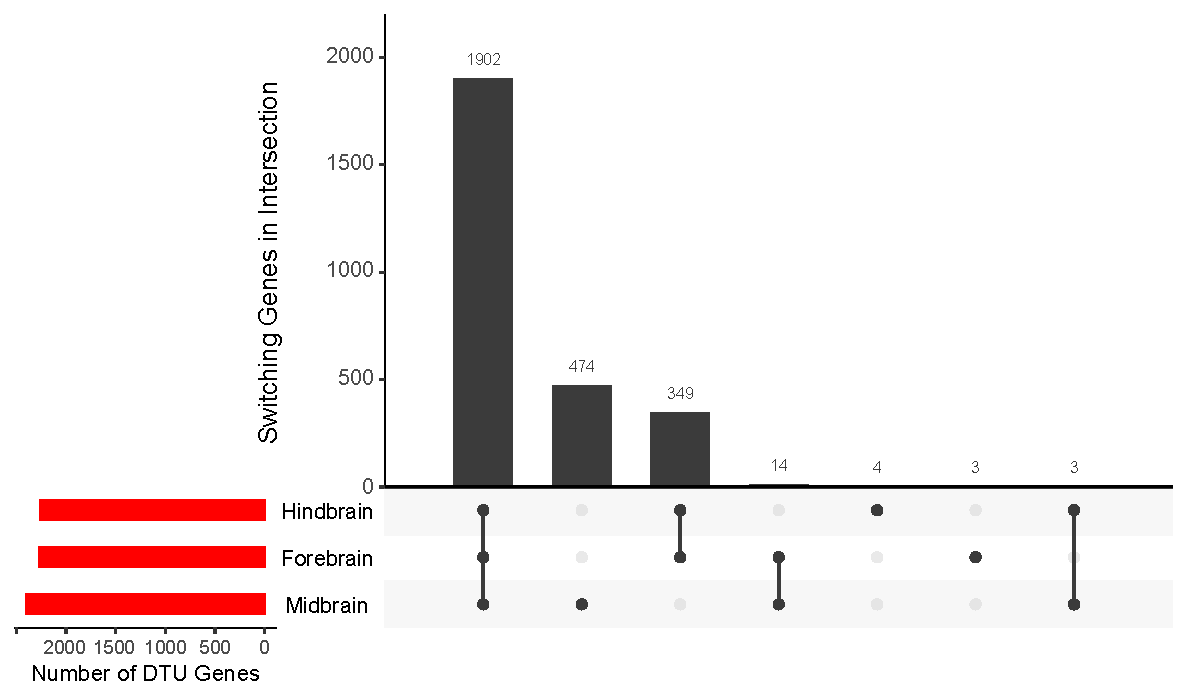
\includegraphics[width=0.88\textwidth]{figure_thesis_dtu_upset.pdf}
\caption{\textbf{Regional intersection of threshold-defined DTU genes.} The sets comprise genes with at least one transcript passing q-value $<0.05$ and $|\dIF|\geq0.10$ in any of the 28 temporal contrasts within forebrain, hindbrain or midbrain. Horizontal bars give total regional set sizes. Filled dots and connecting lines specify each mutually exclusive intersection, and the vertical bar above it gives the number of genes in that intersection. The largest intersection contains 1,902 genes detected in all three regions; 474 genes are detected only in midbrain. A regional set denotes thresholded detection, not strict tissue specificity.}
\label{fig:thesisupset}
\end{figure}

\clearpage
\subsection*{Transcript characteristics and temporal-event summaries}

The following figures present descriptive outputs from the original doctoral analysis; inferential results in the main text use the methods specified in the manuscript.

\begin{figure}[htbp]
\centering
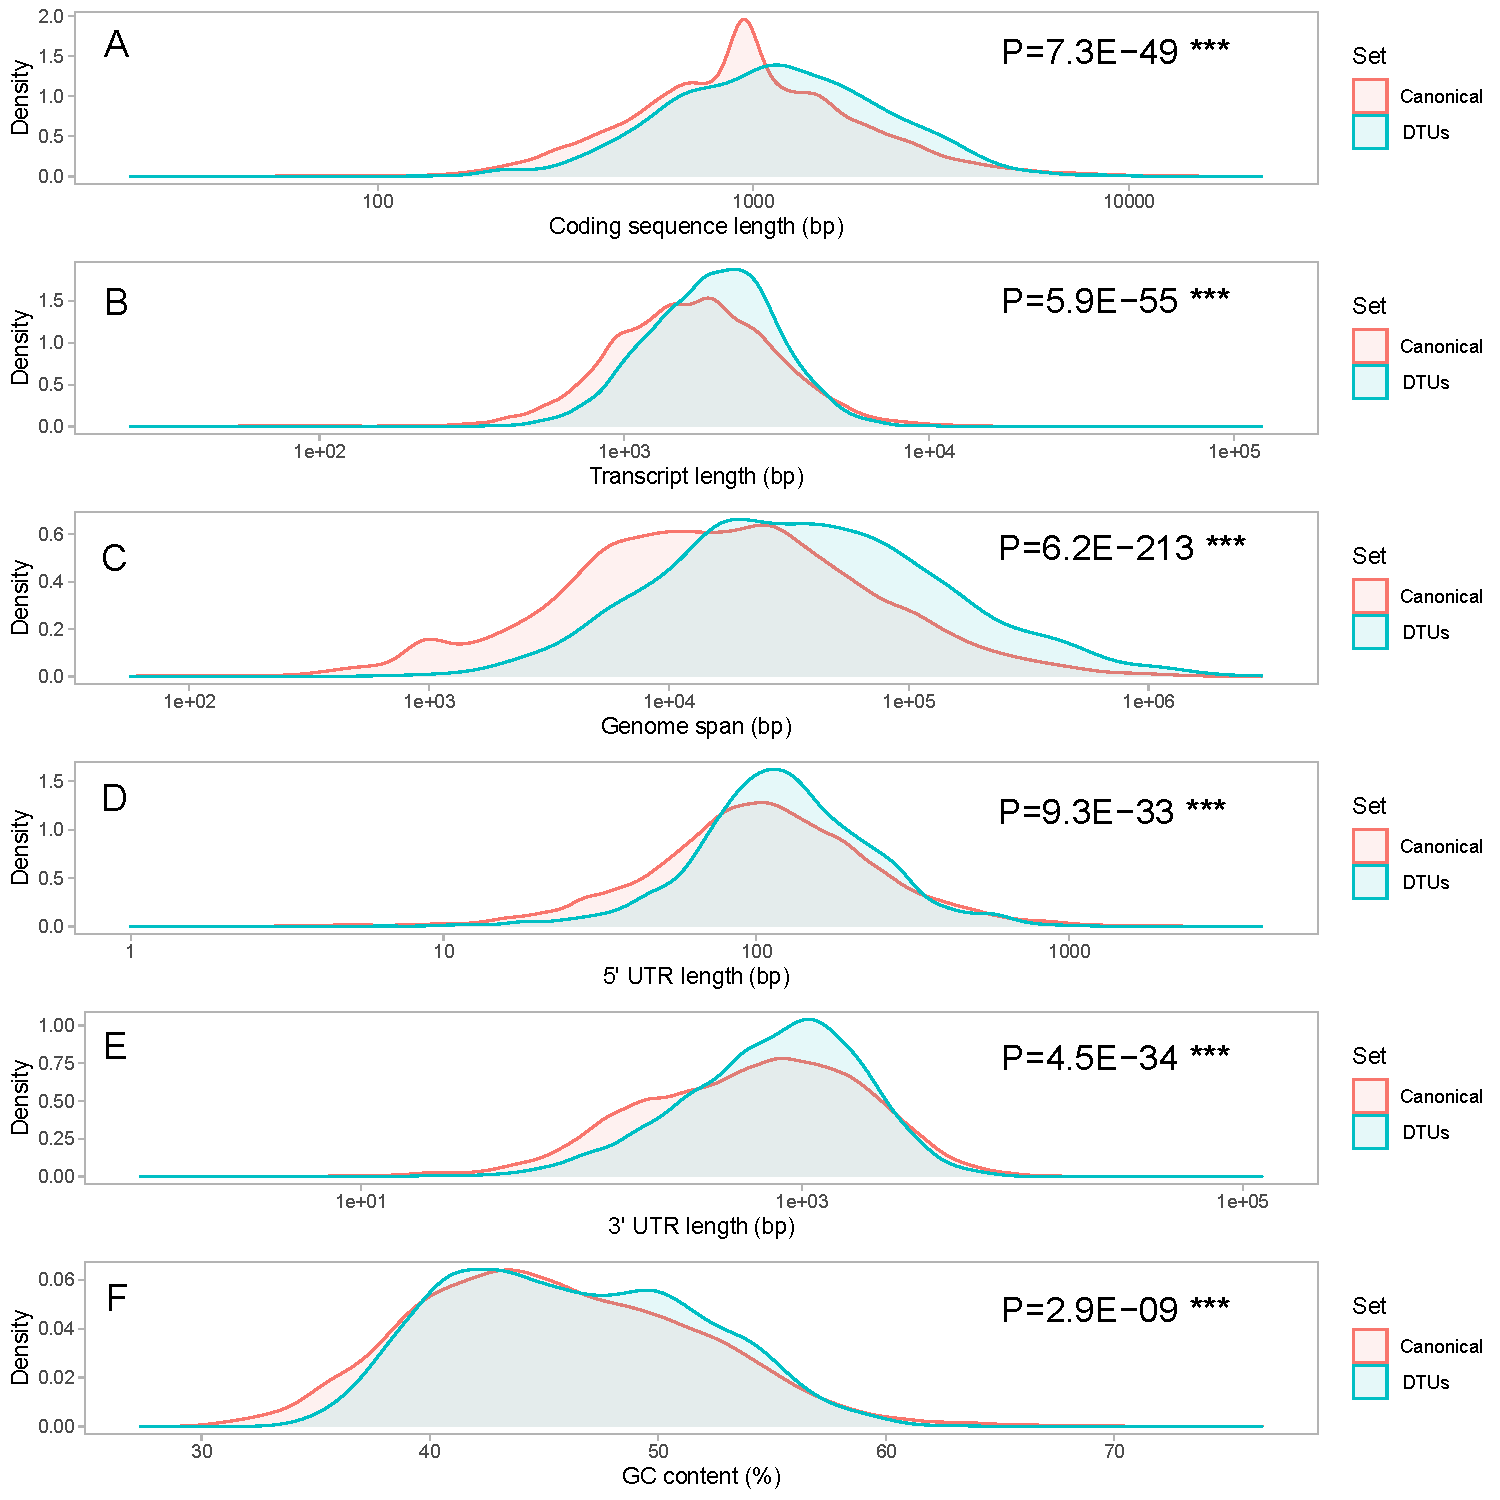
\includegraphics[width=0.80\textwidth]{figureS7_thesis_dtu_attributes.pdf}
\caption{\textbf{Transcript attributes of the DTU catalogue.} Kernel-density distributions compare transcripts in the original threshold-defined DTU catalogue with the original non-DTU comparison universe. Panels show (A) coding-sequence length, (B) total transcript length, (C) genomic span, (D) 5$'$-UTR length, (E) 3$'$-UTR length and (F) GC percentage; length axes are logarithmic where indicated. The $P$-values printed above panels are inherited from the original descriptive workflow; their test identity and multiplicity family were not retained, so they are not used as inferential evidence in the present reanalysis. ``Canonical'' in the inherited legend denotes the non-DTU comparison set rather than a uniquely canonical RefSeq transcript.}
\label{fig:thesisattributes}
\end{figure}

\begin{figure}[htbp]
\centering
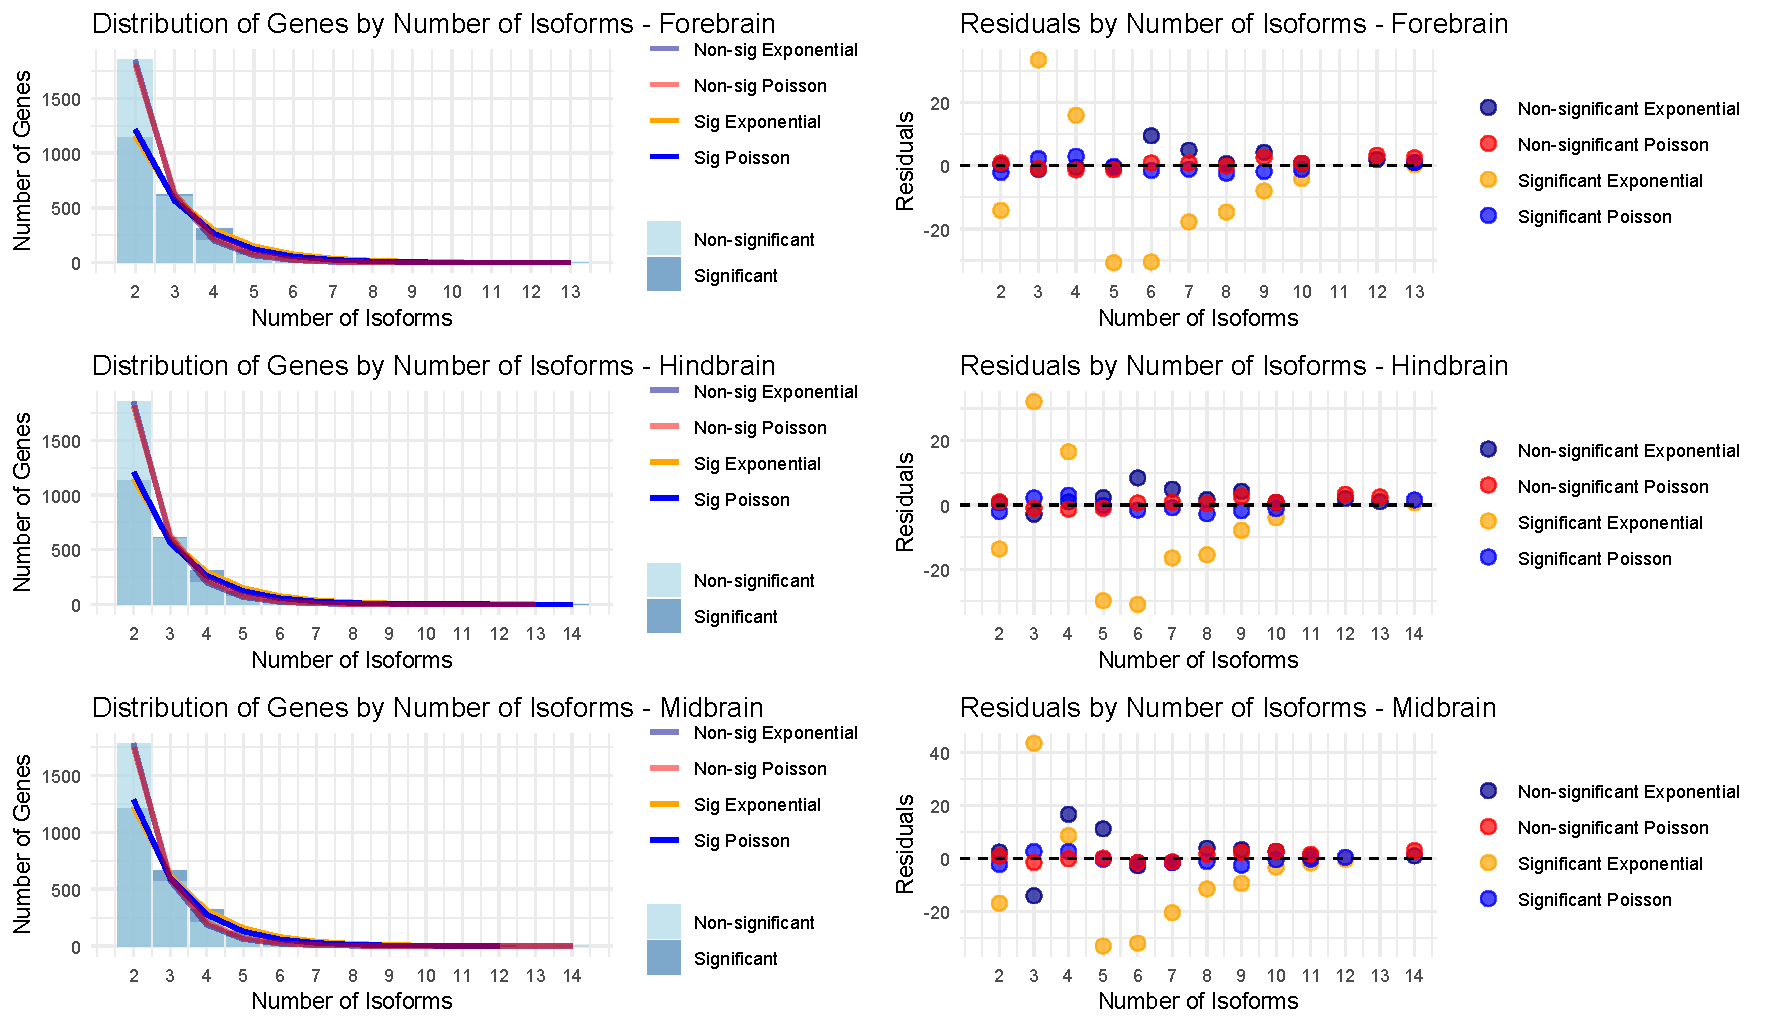
\includegraphics[width=0.84\textwidth]{figure_thesis_isoform_counts.pdf}
\caption{\textbf{Annotated transcript counts in regional DTU and comparison sets.} Rows correspond to forebrain, hindbrain and midbrain. In each row, the left panel gives gene counts by number of annotated transcripts for genes meeting the original regional DTU criteria (``Significant'') and the remaining analysed genes (``Non-significant''); fitted exponential and Poisson curves are overlaid. The right panel shows count residuals from each fitted curve at the same transcript-count values. The display is a descriptive model check of whether genes with more annotated transcripts are over-represented in the DTU catalogue; observations are genes, not individual transcripts.}
\label{fig:thesisisoformcounts}
\end{figure}

\begin{figure}[htbp]
\centering
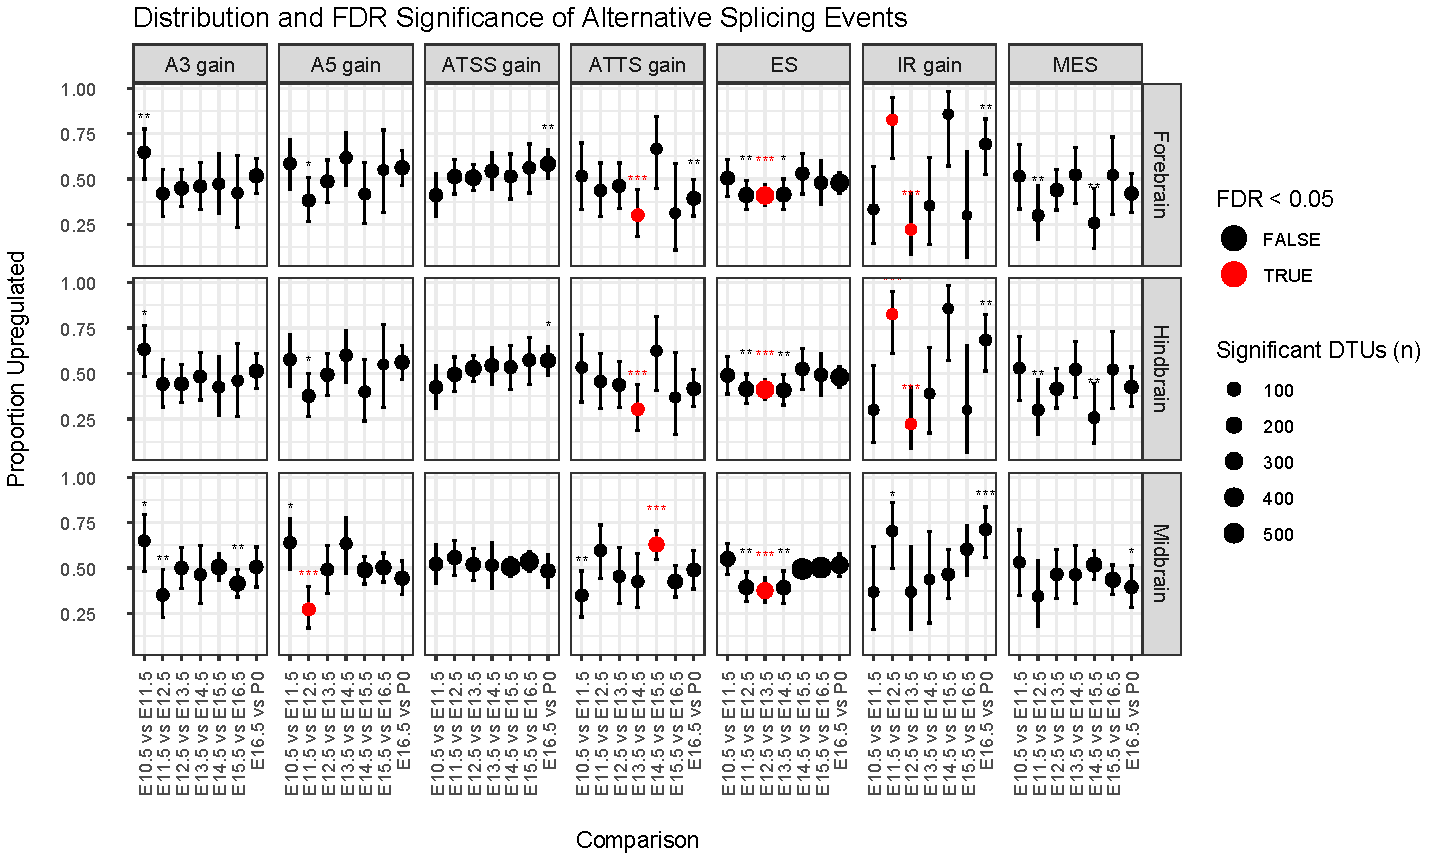
\includegraphics[width=0.86\textwidth]{figure_thesis_temporal_events.pdf}
\caption{\textbf{Temporal distribution of annotated transcript-structure events.} Facets are transcript-structure event classes and the three horizontal groups are forebrain, hindbrain and midbrain. For each adjacent-stage contrast from E10.5--E11.5 through E16.5--P0, a point gives the proportion of significant event-bearing transcripts whose relative usage increased in the stated direction; point size gives the number of significant transcripts and vertical bars are the confidence intervals reported by the original workflow. Red points have the original event-level FDR $<0.05$; asterisks reproduce its significance coding ($*$, $P<0.1$; $**$, $P<0.05$; $***$, $P<0.01$). A3/A5, alternative 3$'$/5$'$ splice-site gain; ATSS/ATTS, alternative transcript start/end gain; ES, exon skipping; IR, intron-retention gain; MES, multiple exon skipping. Event annotations are non-exclusive, and the plot is descriptive rather than part of the systematic episode test.}
\label{fig:thesistemporalevents}
\end{figure}

\begin{figure}[htbp]
\centering
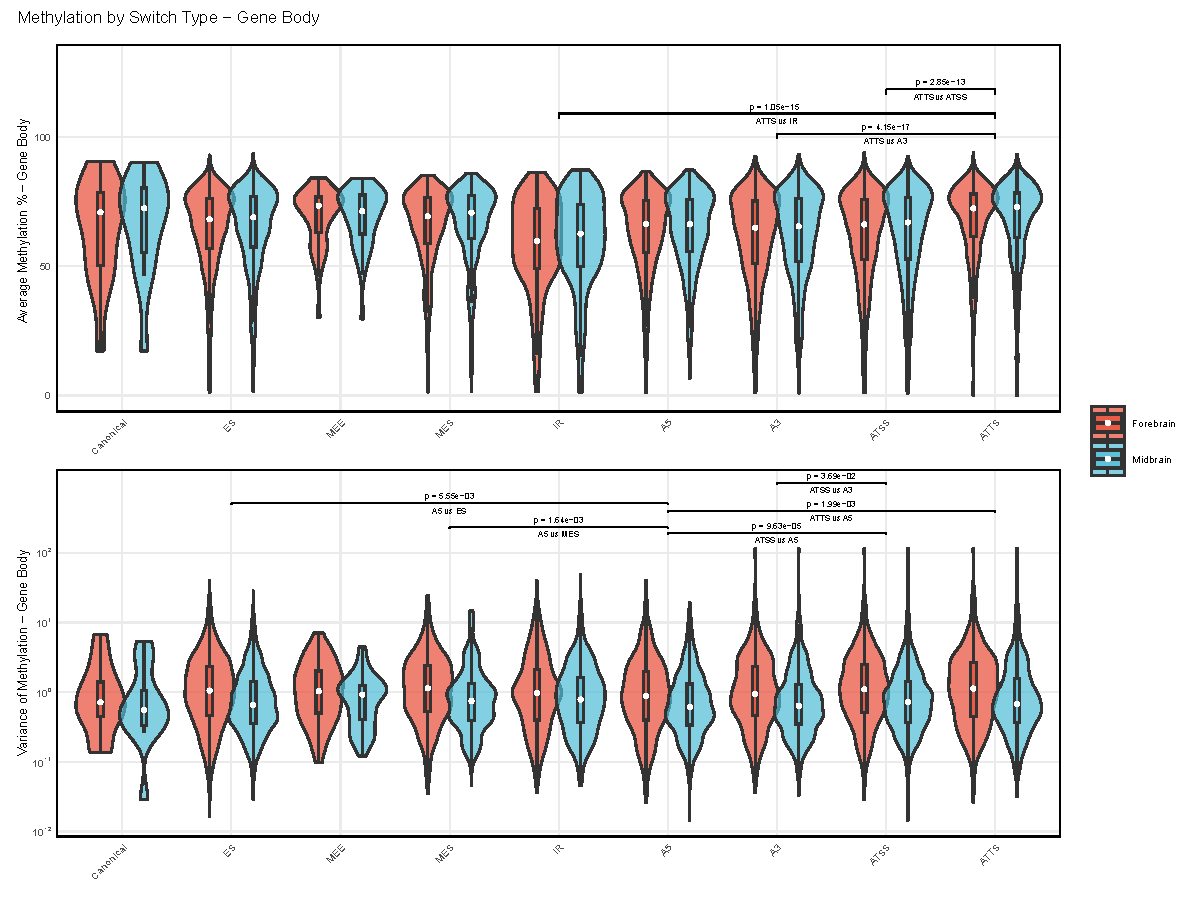
\includegraphics[width=0.90\textwidth]{figureS11_thesis_switch_methylation.pdf}
\caption{\textbf{Gene-body methylation by transcript-event annotation.} Each violin shows the distribution across transcripts in the original selected set, with forebrain and midbrain distinguished by colour. The upper panel uses each transcript's mean gene-body CpG methylation percentage; the lower panel uses its between-sample methylation variance on a logarithmic scale. Groups are ES, MEE, MES, IR, A5, A3, ATSS and ATTS as defined in Figure~S7; annotations are non-exclusive. ``Canonical'' is the inherited label for the comparison group lacking the listed alternative-event annotation, not a uniquely designated RefSeq transcript. Brackets and printed $P$-values are pairwise comparisons from the original workflow and were not included in the analysis-wide methylation correction used in the main text.}
\label{fig:thesisswitchmeth}
\end{figure}

\begin{figure}[htbp]
\centering
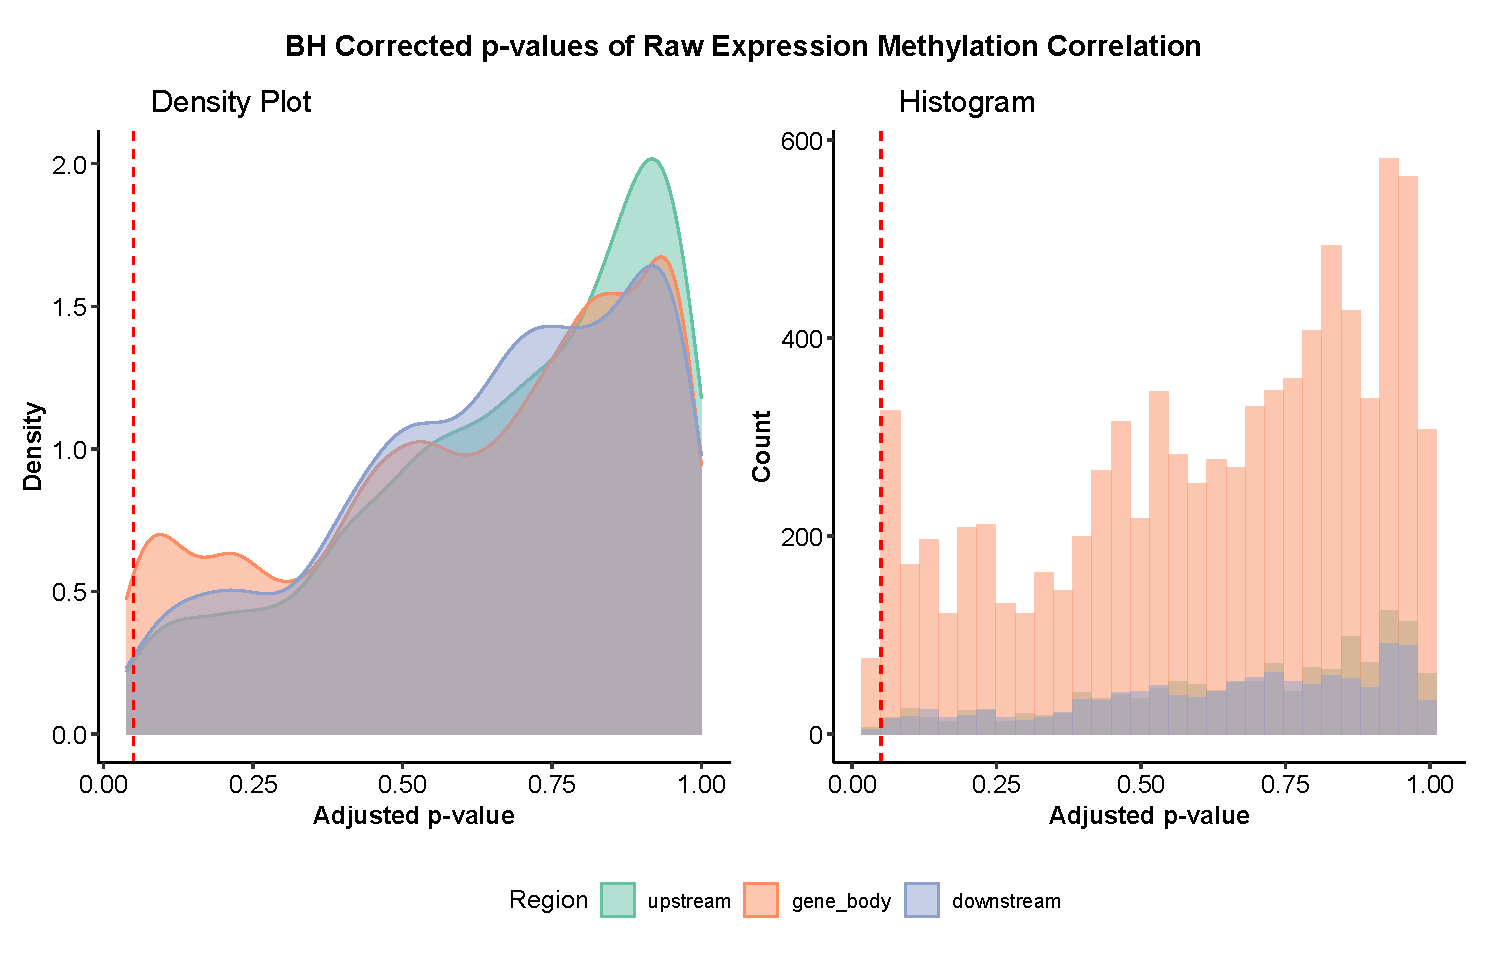
\includegraphics[width=0.90\textwidth]{figure_thesis_archived_bh.pdf}
\caption{\textbf{Methylation associations with absolute transcript expression in the original workflow.} The displayed observations combine forebrain and midbrain transcript--region associations that were prefiltered at nominal correlation $P<0.05$. The left panel is a kernel-density estimate and the right panel the corresponding histogram of Benjamini--Hochberg-adjusted $P$-values; colour denotes the 6-kb upstream window, gene body with 2-kb margins or 6-kb downstream window. Adjustment was performed separately within each genomic-region class after nominal prefiltering. Consequently, these values are conditional, region-wise summaries and are not the analysis-wide q-values reported in the main reanalysis.}
\label{fig:thesisrawbh}
\end{figure}

\begin{figure}[htbp]
\centering
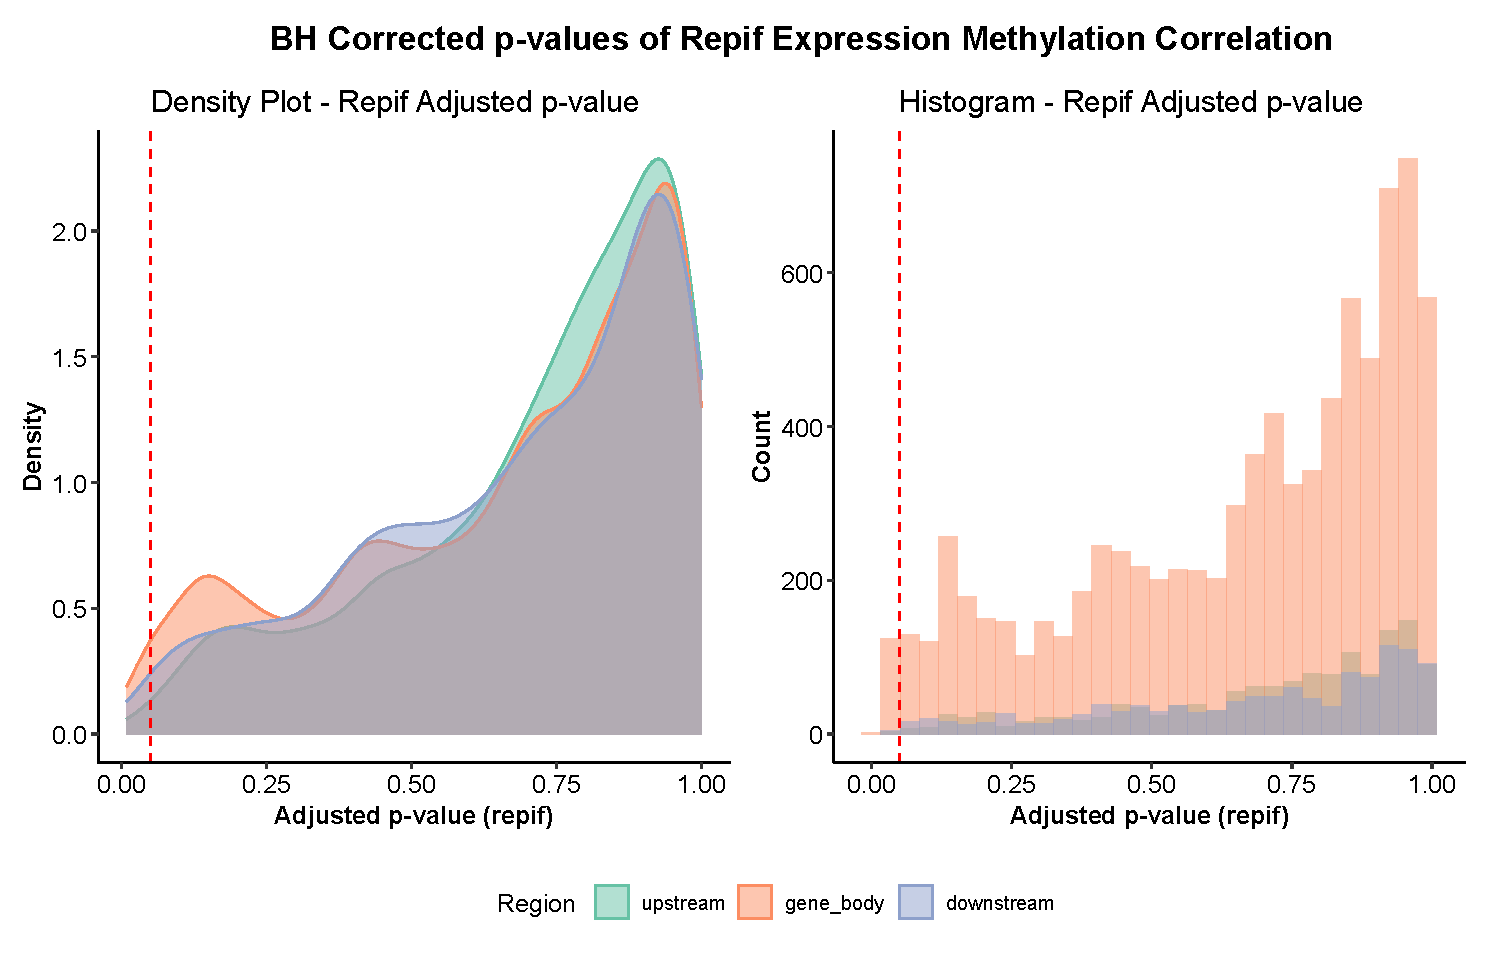
\includegraphics[width=0.90\textwidth]{figure_thesis_archived_repif_bh.pdf}
\caption{\textbf{Methylation associations with relative transcript fraction in the original workflow.} The displayed observations combine forebrain and midbrain transcript--region associations that were prefiltered at nominal correlation $P<0.05$. The left panel is a kernel-density estimate and the right panel the corresponding histogram of Benjamini--Hochberg-adjusted $P$-values; colour denotes the 6-kb upstream window, gene body with 2-kb margins or 6-kb downstream window. Adjustment was performed separately within each genomic-region class after nominal prefiltering. Relative transcript fraction is the transcript abundance divided by the summed abundance of retained transcripts from the same gene. These conditional, region-wise values are distinct from the analysis-wide q-values in the main reanalysis.}
\label{fig:thesisrepifbh}
\end{figure}

\begin{figure}[htbp]
\centering
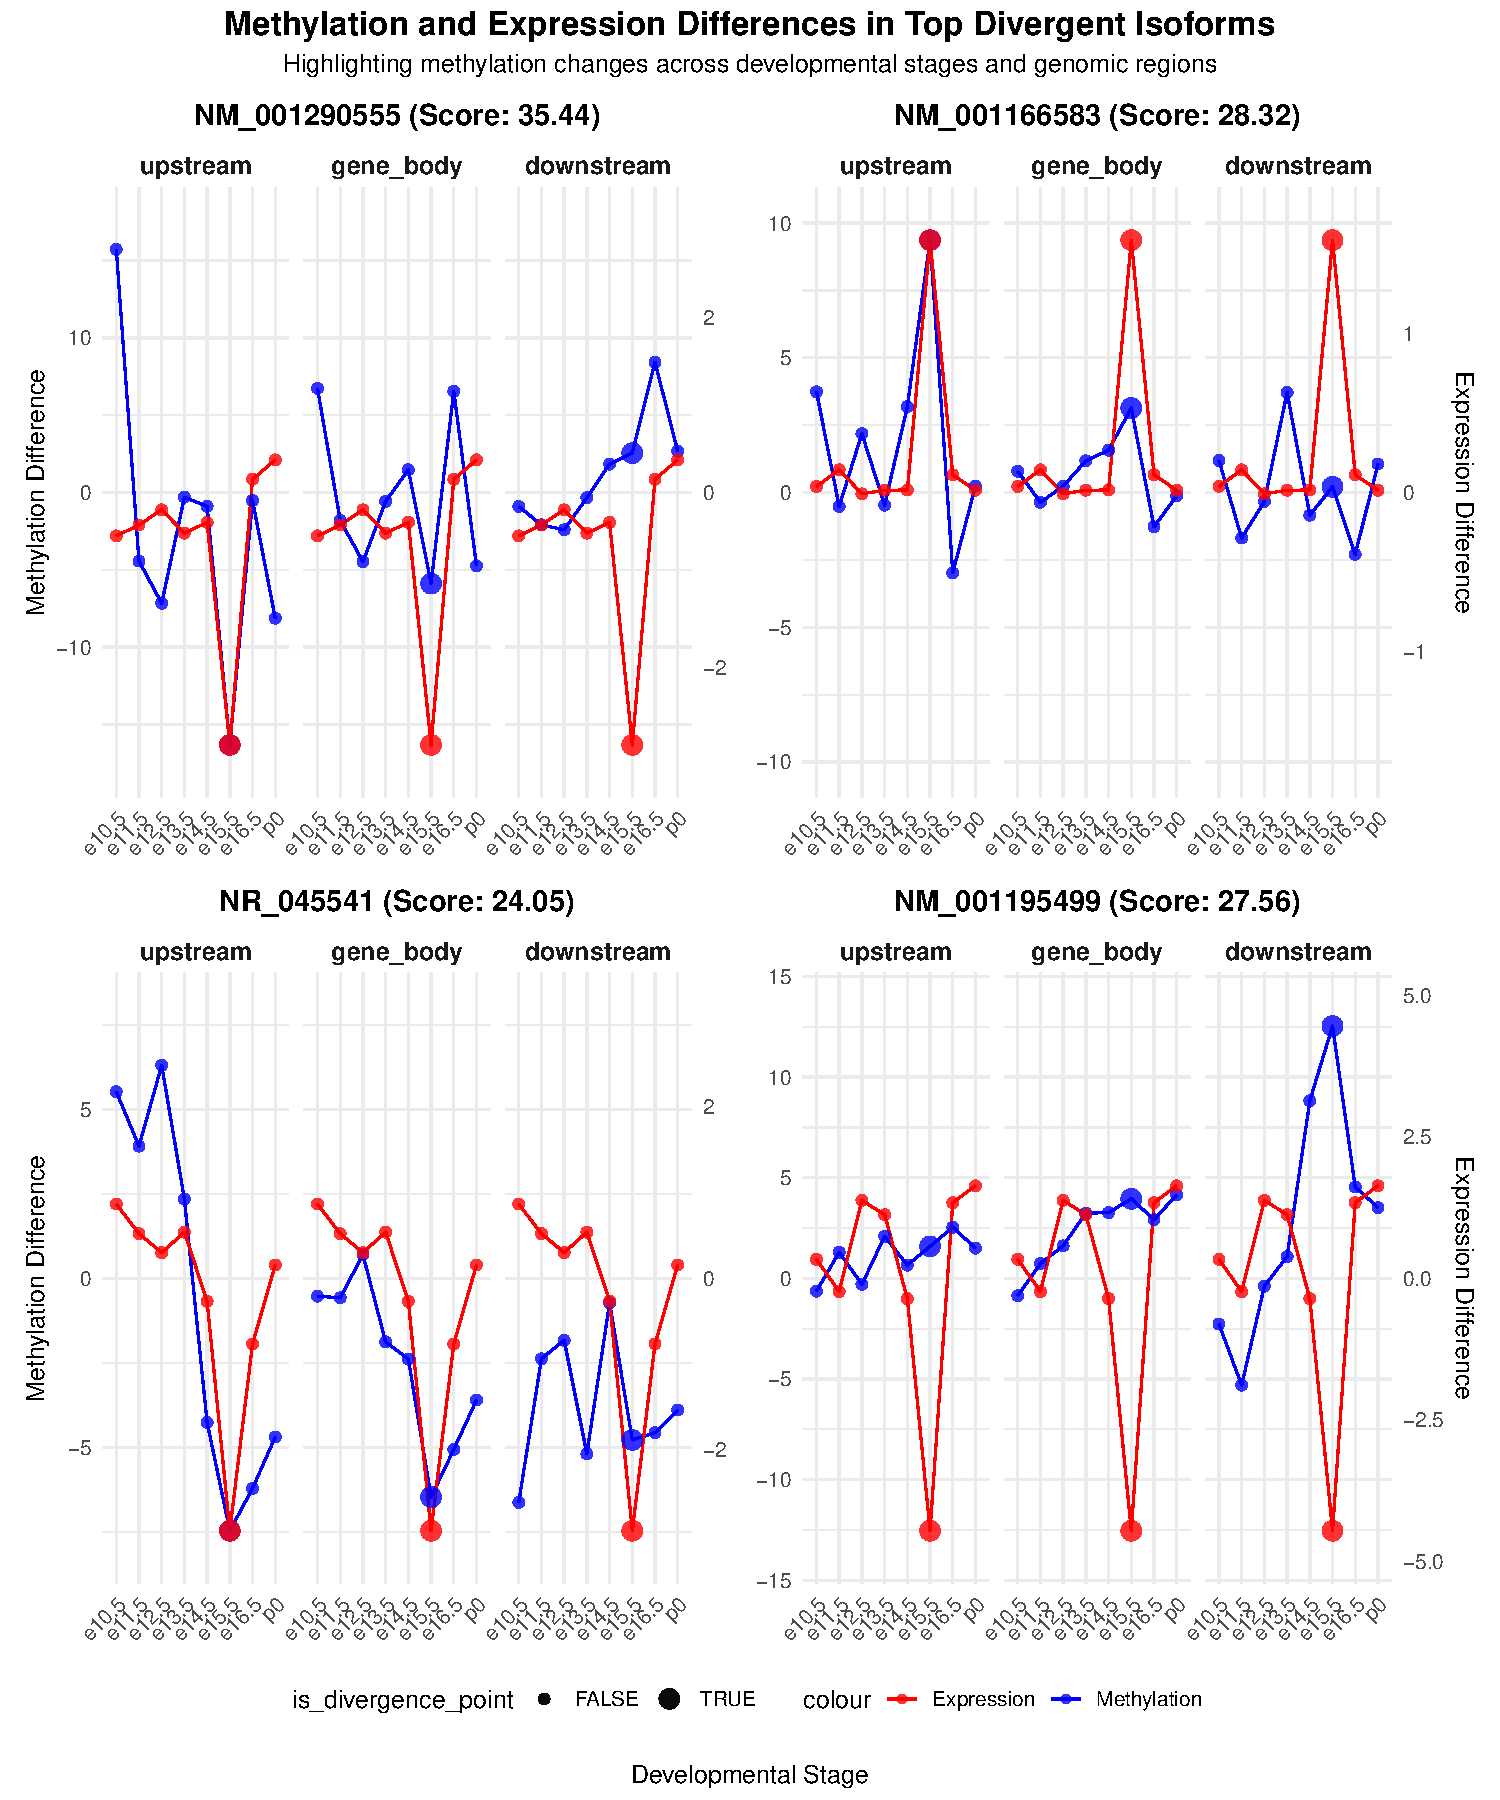
\includegraphics[width=0.92\textwidth]{figure_thesis_weighted_candidates.pdf}
\caption{\textbf{Methylation-weighted transcript candidates from the original ranking.} Rows show \textit{Pja1} NM\_001290555, \textit{Fam122b} NM\_001166583, \textit{Oprl1} NR\_045541 and \textit{Dclk2} NM\_001195499; columns show the 6-kb upstream window, gene body with 2-kb margins and 6-kb downstream window. Across E10.5--P0, blue and red trajectories are the midbrain-minus-forebrain methylation and transcript-expression differences, respectively, plotted on separate y-axis scales. Larger points identify stages classified as expression-divergence points by the original heuristic. ``Score'' is the inherited methylation-weighted divergence score used to rank 891 transcripts; it is not an analysis-wide test statistic or q-value.}
\label{fig:thesisweighted}
\end{figure}

\clearpage
\subsection*{Chromatin and methylation context}

These figures present exploratory chromatin-state and methylation summaries for the original transcript sets selected by the doctoral workflow before the analysis-wide reconstruction.

\begin{figure}[htbp]
\centering
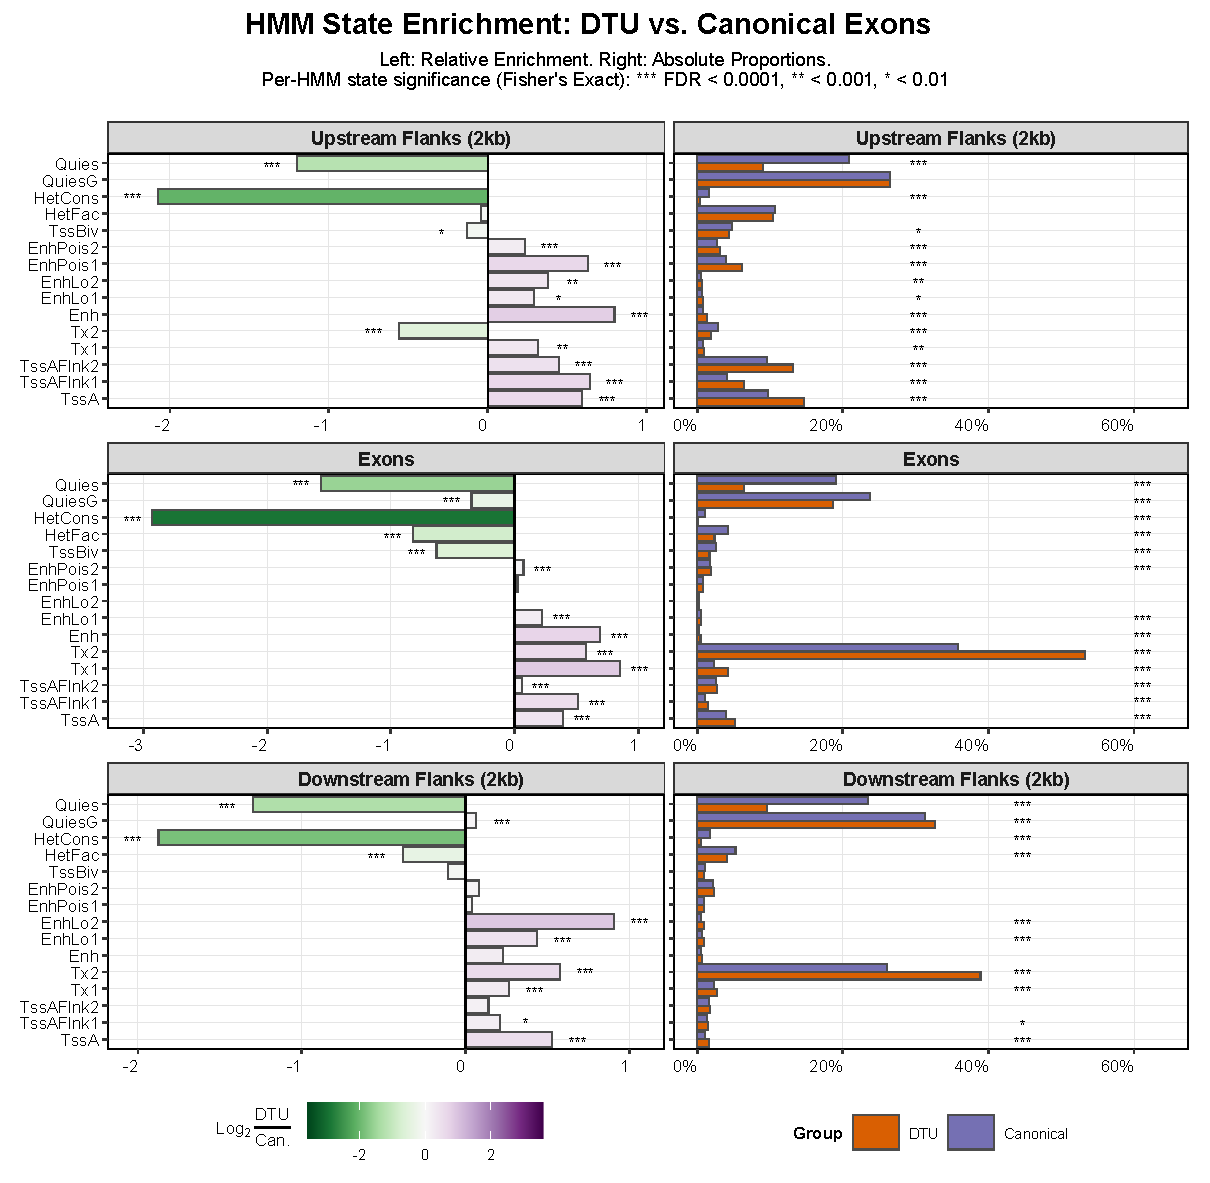
\includegraphics[width=0.94\textwidth]{figureS7_thesis_hmm_enrichment.pdf}
\caption{\textbf{Chromatin-state enrichment around DTU and comparison exons.} The analysis uses the 15-state E13.5 forebrain chromatin hidden Markov model. Rows are chromatin states and columns are the 2-kb upstream flank, exon and 2-kb downstream flank. Left panels show $\log_2$ enrichment of state overlap in the original DTU exon set relative to the non-DTU comparison set; right panels show the absolute percentage of features overlapping each state, with colour distinguishing the two sets. ``Canonical'' is the inherited label for the non-DTU comparison exons. Asterisks report per-state Fisher exact tests after FDR correction ($*$, FDR $<0.01$; $**$, FDR $<0.001$; $***$, FDR $<0.0001$).}
\label{fig:thesishmmenrichment}
\end{figure}

\begin{figure}[htbp]
\centering
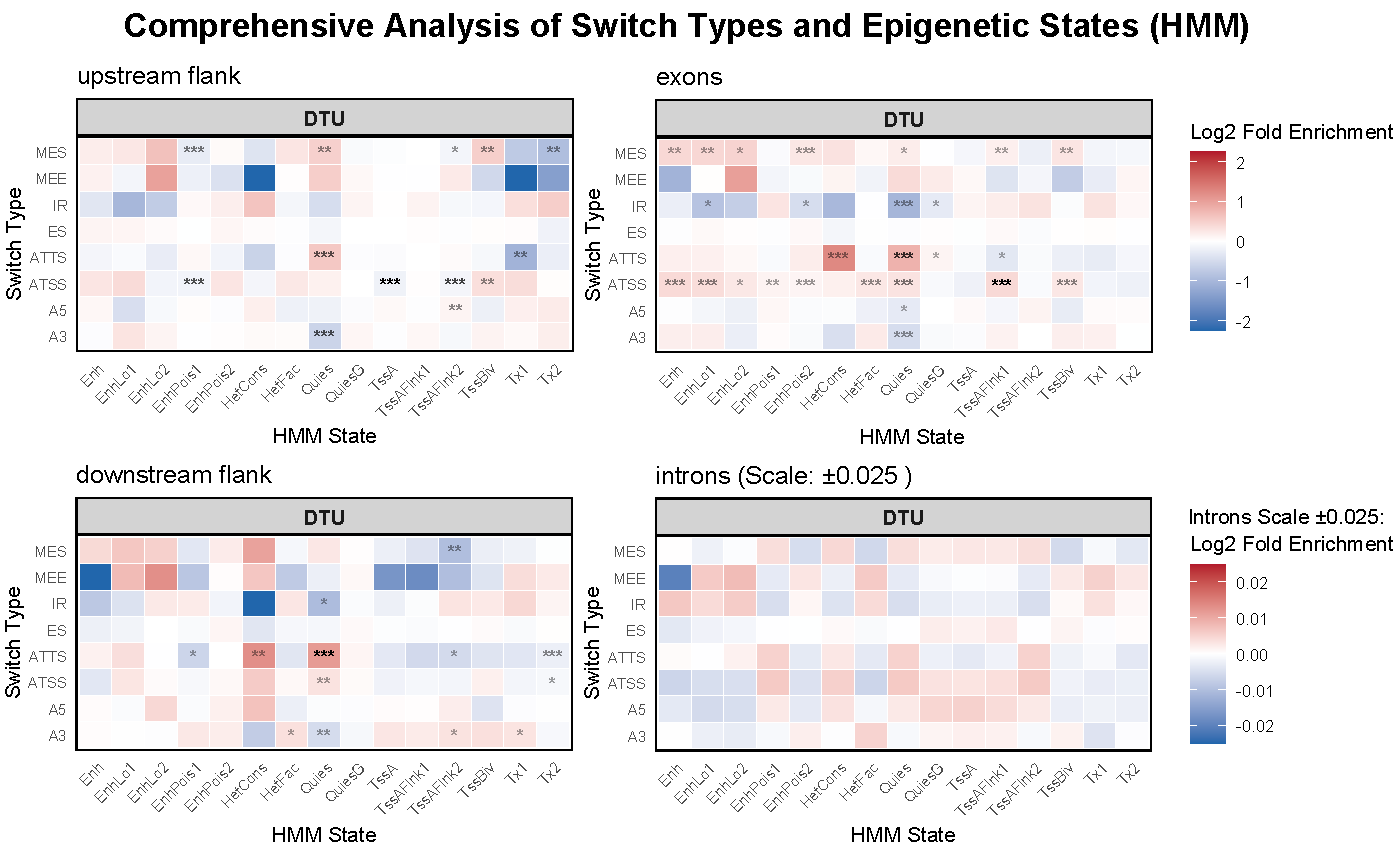
\includegraphics[width=0.94\textwidth]{figureS8_thesis_switch_hmm.pdf}
\caption{\textbf{Chromatin-state profiles by transcript-event annotation.} Four heatmaps show $\log_2$ enrichment of the 15 E13.5 forebrain hidden-Markov chromatin states in exons, introns, 2-kb upstream flanks and 2-kb downstream flanks. Rows are the pooled DTU set and the ES, MEE, MES, IR, A5, A3, ATSS and ATTS annotation groups defined in Figure~S7; columns are the named chromatin states. Enrichment is relative to the original non-DTU comparison set, with positive values indicating over-representation. The intron panel uses the narrower scale printed in the figure ($\pm0.025$); the other panels use the common $\log_2$ scale. Asterisks reproduce the original FDR-coded state comparisons ($*$, FDR $<0.01$; $**$, FDR $<0.001$; $***$, FDR $<0.0001$).}
\label{fig:thesisswitchhmm}
\end{figure}

\begin{figure}[htbp]
\centering
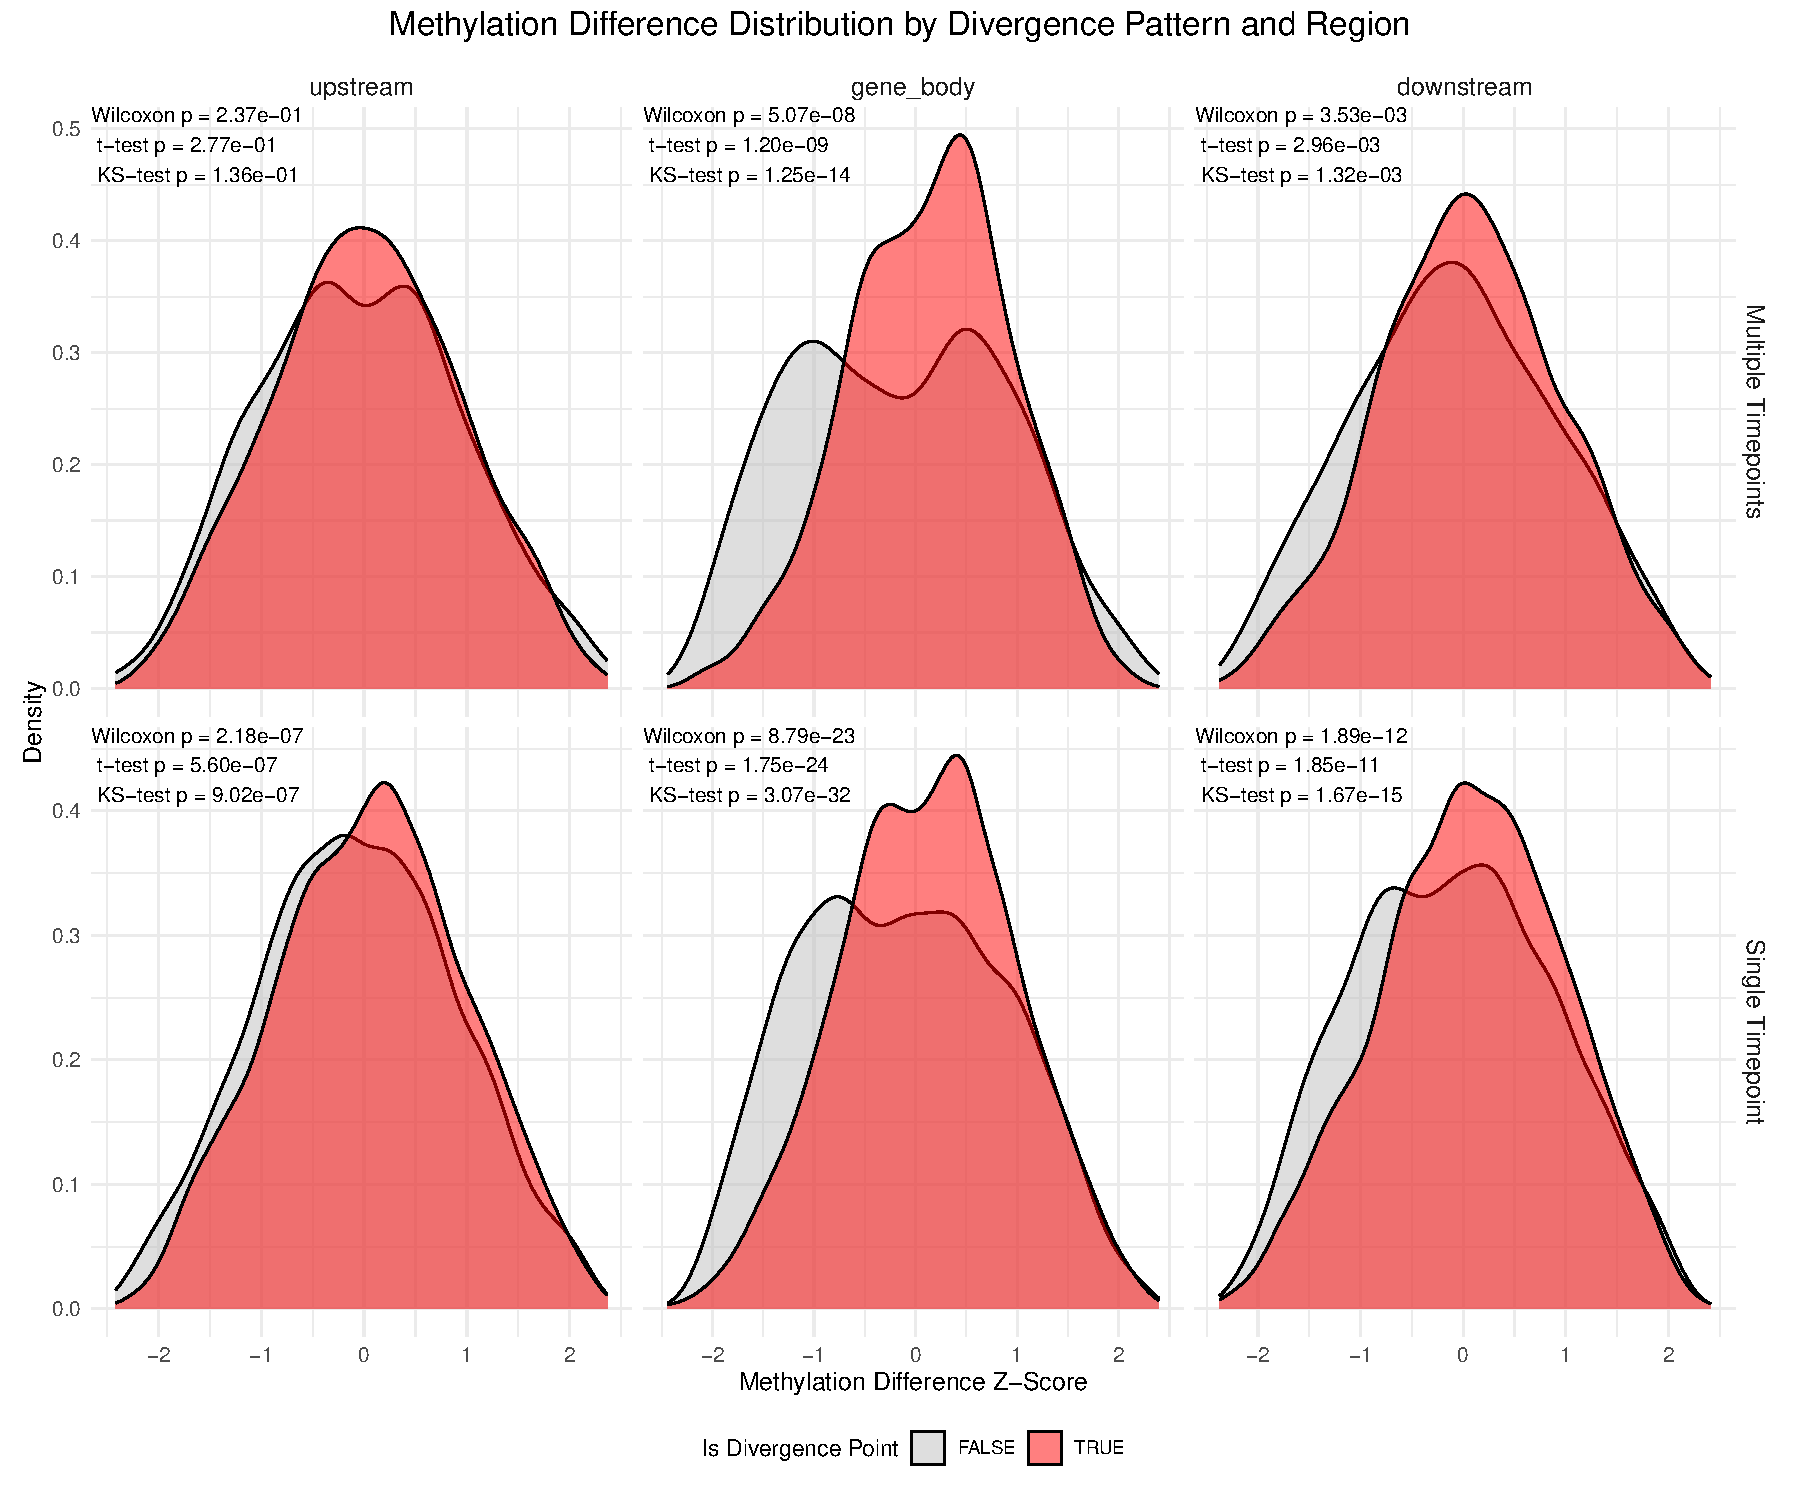
\includegraphics[width=0.94\textwidth]{figureS9_thesis_methylation_divergence.pdf}
\caption{\textbf{Methylation differences at divergent and non-divergent stages.} The observations derive from 891 transcripts selected by the original forebrain--midbrain expression-divergence heuristic. Columns are the 6-kb upstream window, gene body with 2-kb margins and 6-kb downstream window; rows separate transcripts divergent at multiple stages from those divergent at one stage. Within each facet, density curves compare transcript--stage methylation-difference Z-scores at stages labelled as expression-divergent (red) with the remaining stages (grey). The Z-score standardises the midbrain-minus-forebrain methylation difference within each transcript and genomic region across stages. Printed values are nominal two-sided Wilcoxon rank-sum, t-test and Kolmogorov--Smirnov $P$-values from the original workflow; no multiplicity correction across the six facets and three tests is encoded in the figure.}
\label{fig:thesismethdivergence}
\end{figure}

\end{document}
